\documentclass{article}
\usepackage{icais_conference,times}
\input{math_commands.tex}

\usepackage{amsmath,amssymb,array,booktabs,graphicx,multirow,xspace,float}
\usepackage{algorithm,algpseudocode}
\usepackage{hyperref}
\hypersetup{colorlinks=true,linkcolor=blue!70!black,citecolor=green!60!black,urlcolor=red!60!black}
\usepackage{url}

\setlength{\textfloatsep}{4pt plus 1pt minus 1pt}
\setlength{\floatsep}{3pt plus 1pt minus 1pt}
\setlength{\intextsep}{4pt plus 1pt minus 1pt}
\setlength{\abovecaptionskip}{2pt}
\setlength{\belowcaptionskip}{0pt}
\setlength{\abovedisplayskip}{6pt plus 2pt minus 2pt}
\setlength{\belowdisplayskip}{6pt plus 2pt minus 2pt}

\graphicspath{{paper_assets/}}
\newcommand{\ours}{\textsc{Auditable Discovery Loop}}
\newcommand{\resfilter}{Residual Filter (RF)\xspace}
\newcommand{\respenalty}{Residual Penalty (RP)\xspace}
\newcommand{\nominalonly}{Nominal-only\xspace}
\newcommand{\graphcbf}{Graph-CBF adaptation\xspace}
\newcommand{\mappoadapt}{MAPPO adaptation\xspace}
\newcommand{\dcbf}{distributed CBF\xspace}
\newcolumntype{L}[1]{>{\raggedright\arraybackslash}p{#1}}

\title{Auditable AI-assisted discovery of a transferable safety mechanism for multi-UAV control}
\author{Anonymous Authors}

% Keep \iclrfinalcopy commented for double-blind review.
%\iclrfinalcopy

\begin{document}
\maketitle

\begin{abstract}
AI systems can modify code, run experiments and draft scientific text, yet an improved score does not identify a mechanism or its failure boundary. We introduce an auditable discovery loop that locks controller definitions, paired disturbances, terminal labels, aggregation rules and source artifacts before admitting claims. A discrete screen first tests whether rejecting predicted barrier violations explains small-team gains; a continuous graph-CBF experiment then tests the same mechanism under a different action space. Across 44,000 continuous episodes, collision falls from 100\% to 12.6\% at $N=3$ and to 31.0\% at $N=5$, while team success rises from 0\% to 29.8\% and 15.6\%. The effect weakens with scale and reaches 100\% collision in a withheld dense $N=12$ layout. Four hundred PX4 software-in-the-loop runs establish command-chain and telemetry integrity over a 3-s Offboard window. The resulting evidence supports a bounded, falsifiable mechanism claim rather than scalable or deployment-level safety.
\end{abstract}

\section{Introduction}

Multi-UAV navigation is a coupled safety problem: every vehicle must make progress while avoiding other vehicles, moving obstacles and geometry under disturbance and communication loss. Expected-return learning can trade a rare collision against progress, whereas control-barrier methods impose local constraints on admissible motion \citep{ames2017cbf,garg2024safe}. Graph policies and neural certificates extend these ideas to variable neighbourhoods \citep{qin2021neural,zhang2025gcbfplus,zhang2025dgppo,nayak2023informarl}, but dense scenes expose a persistent ambiguity: an apparent safety gain may arise from the barrier, from a shared nominal controller, or from the evaluator selecting favourable outcomes.

When an AI agent generates candidates, chooses checkpoints and writes the result, this ambiguity is amplified. Autonomous-science systems demonstrate that code and experiments can be orchestrated end to end \citep{yang2024sweagent,lu2024aiscientist}. Our control condition is reconstruction from failures that were not selected away. We therefore use one evaluator with mutually exclusive terminal labels, paired seeds, and episode records linked to source artifacts. The automated loop executes these locked operations; human researchers retain the research question, evidence boundary and final interpretation.

This procedure isolates a mechanism-level signal and tests where it transfers. Stage I screens six arms around one unchanged goal-progress controller, with an independent safety-budget sweep and one-at-a-time perturbations. Stage II changes the implementation to simultaneous continuous graph control, preserving only the hypothesis that predicted barrier violations should be rejected. We evaluate scale, information visibility and an external flight-stack interface separately. The contribution is a traceable path from generated hypothesis to positive evidence, falsification and an explicit boundary, not a new universally safe controller.

Figure~\ref{fig:loop} situates these contributions within the full discovery workflow, separating human scientific control from automated execution and showing how the evidence contract links mechanism screening, paired evaluation, and claim revision.

\begin{figure}[!t]
\centering
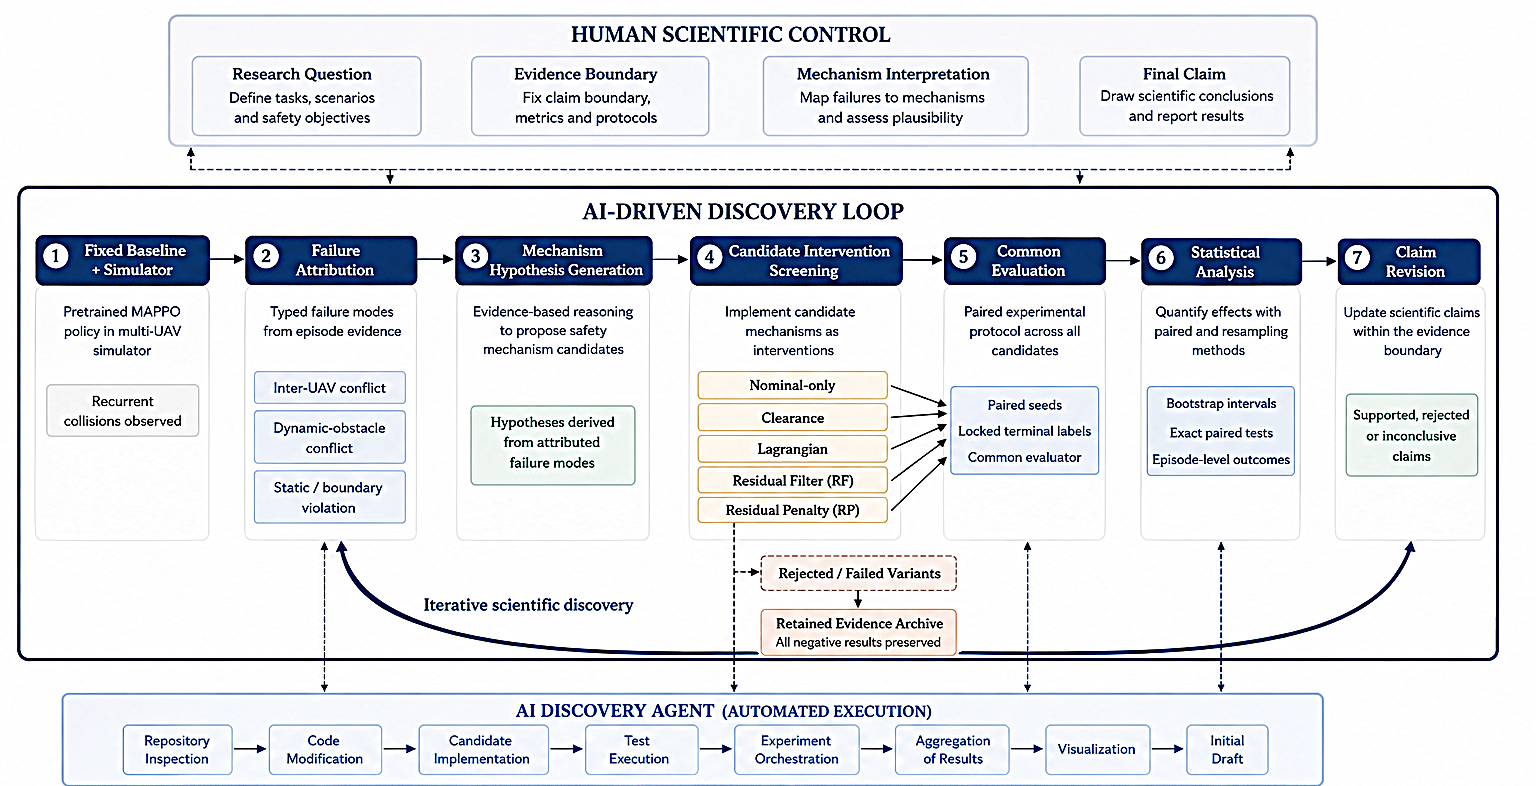
\includegraphics[width=0.985\linewidth]{fig01_compact.png}
\caption{\textbf{Auditable AI-assisted discovery loop.} Human researchers set the question, evidence boundary, labels, interpretation, and final claim. The automated loop executes attribution, candidate implementation, common testing, paired evaluation, aggregation, visualization, and initial drafting. The evidence contract binds locked controller definitions, terminal labels, independently recomputable aggregates, and source artifacts across all stages. Failed candidates remain visible.}
\label{fig:loop}
\end{figure}

\section{The auditable discovery loop}

\subsection{Problem setting and terminal outcomes}
Vehicle $i$ has position $p_i\in\mathbb R^3$, velocity $v_i$, goal $g_i$, and observation $o_i$. Stage I uses seven discrete actions at $\Delta t=0.25$~s; Stage II uses simultaneous commands $u_i\in[-1,1]^3$ with 2.0~m/s speed and 2.0~m/s$^2$ acceleration limits. Five scenarios vary static layout, moving obstacles, density, wind, and communication dropout; a withheld dense $N=12$ layout tests out-of-distribution scale.

The safety proxy $c(x)$ is the clipped maximum normalized violation of agent--agent, dynamic-obstacle, and static-clearance budgets. It guides candidate design but never supplies terminal labels. Collision means separation below $0.55$~m or penetration of geometry/boundaries; team success requires every goal reached collision-free within 128 steps, leaving timeout as a distinct outcome. Continuous actors receive graphs of relative kinematics, goals, node type, and communication state. Local actors mask nodes beyond 6~m and experience packet dropout; privileged actors observe all nodes. Only the critic uses global state during training.

\subsection{Evidence contract}
\noindent\textbf{Definition 1 (Evidence contract).} A reported claim is admissible when its controller definition, paired evaluation protocol, episode-level terminal labels, aggregation rule, and source artifact can be independently recomputed. Natural-language interpretation cannot modify terminal labels. Candidates rejected by the shared evaluator remain in the decision record.

One evaluator computes terminal labels for every arm, preventing candidates from receiving credit for lowering $c(x)$ while leaving terminal collisions unchanged and exposing the full comparison set rather than favorable variants only.

\subsection{Stage I: discrete mechanism screen}
Typed failure attribution separates static and boundary contacts from inter-UAV conflicts, narrowing the intervention space to four mechanisms around one shared goal-directed nominal controller. The nominal-only arm tests whether one-step progress alone reproduces candidate gains. MAPPO is the trained failure reference motivating this diagnostic screen, not an algorithm-equivalent competitor to deterministic variants.

\begin{table}[t]
\caption{Stage-I variants and the screening question answered by each arm. The four deterministic mechanisms share one nominal controller.}
\label{tab:controllers}
\centering
\small
\begin{tabular}{L{0.19\linewidth}L{0.31\linewidth}L{0.39\linewidth}}
\toprule
Variant & Intervention & Screening question \\
\midrule
MAPPO & Pretrained actor & Does the original learned policy solve the task? \\
Nominal-only & Goal-progress score & Does the nominal controller explain the result? \\
Clearance score & Progress plus clearance & Is local clearance sufficient? \\
Lagrangian & Adaptive $\lambda c(x^+)$ & Can one soft cost balance progress and safety? \\
RF & Hard residual filter & Does rejecting predicted violations help? \\
RP & Soft residual penalty & Does residual penalization preserve progress? \\
\bottomrule
\end{tabular}
\end{table}

For a candidate action $a$ with predicted next state $x^+$, the screen defines
\begin{equation}
\rho(x,a)=\frac{c(x^+)-c(x)}{\Delta t}+\alpha c(x),\qquad \alpha=1.
\label{eq:residual}
\end{equation}
RF admits actions with $\rho\leq0$ and adequate clearance, then selects the one with greatest goal progress. If none is admissible it minimizes predicted cost before progress. RP retains all actions and ranks them by
\begin{equation}
s(a)=\beta_g\Delta_g-\beta_\rho\max(\rho+\epsilon,0)-\beta_n\mathbb{1}[a\neq a_{\rm nom}]+\beta_c\min(d_{\min},d_{\max}),
\label{eq:rp_score}
\end{equation}
where $\Delta_g$ is one-step goal progress and $d_{\min}$ is predicted minimum clearance. Both variants query simulator geometry, making Stage I a full-state mechanism diagnosis rather than a deployable decentralized policy. The coefficients are hand-set for scale and are reported in Appendix~\ref{app:rp}; they are perturbed one at a time rather than treated as optimized values.

\subsection{Stage II: continuous graph-CBF adaptation}
Stage II translates the RF hypothesis from Stage I into simultaneous continuous control: predicted barrier violations are rejected, but the action space and observation model now change. For each agent, node embeddings $z_{ij}$ are combined with one mean neighborhood message,
\begin{equation}
z_{ij}=\sigma(W_x x_{ij}),\qquad
m_i=\frac{\sum_j A_{ij}z_{ij}}{\max(\sum_j A_{ij},1)},\qquad
\tilde z_i=\sigma(W_m[z_{i0},m_i]).
\label{eq:message}
\end{equation}
The actor adds a bounded learned residual to the unit goal direction and outputs a Gaussian tanh policy. A global-state critic supplies centralized value estimates. An auxiliary barrier head regresses the normalized clearance target $y_{ij}=\operatorname{clip}((d_{ij}-d_s)/d_s,-1,2)$ on active non-self nodes.

The executed graph-CBF command is obtained by projecting the desired velocity $u_i^{\rm des}$ onto local pairwise barrier half-spaces. For relative position $r_{ij}=p_j-p_i$, neighbor velocity $v_j$, and robust radius $d_r$, define $h_{ij}=\lVert r_{ij}\rVert^2-d_r^2$. The admissible command satisfies
\begin{equation}
r_{ij}^{\top}u_i\le r_{ij}^{\top}v_j+0.65h_{ij}.
\label{eq:halfspace}
\end{equation}
Four alternating projection passes enforce all active constraints; an unresolved violation triggers hover. The graph-CBF loss is
\begin{equation}
\mathcal L=\mathcal L_{\rm PPO}+0.5\mathcal L_V-0.005\mathcal H+0.8\mathcal L_{\rm barrier}.
\label{eq:loss}
\end{equation}
The compute-matched MAPPO adaptation uses the same continuous nominal-residual actor, global critic, PPO optimizer, and training cells, but flattens the padded node tensor and omits graph message passing, the auxiliary barrier loss, and the projection. A non-learned distributed-CBF baseline applies Eq.~\ref{eq:halfspace} to the direct goal command. Local and privileged graph-CBF variants differ only in actor visibility.

The cross-stage correspondence is mechanistic, not algorithmic: RF and the graph-CBF adaptation both reject predicted barrier violations, but one enumerates discrete actions using full simulator geometry whereas the other projects simultaneous continuous commands from local graph observations.

\section{Methods}

\subsection{AI system and contribution mapping}
The automated loop was driven by the OpenAI Codex model \textbf{GPT-5.6-sol}, version 5.6 (model identifier ``gpt-5.6-sol'', accessed 26 August 2026). Its operational contributions were: repository and provenance inspection; candidate implementation and smoke testing; experiment orchestration and checkpoint bookkeeping; aggregation, plotting and discrepancy checks; and an initial manuscript draft. Human researchers selected the research question, fixed terminal labels and evidence boundaries, reviewed the mechanism mapping and statistics, and approved the final interpretation. No model output could alter the evaluator or relabel an episode after observing its outcome.

\subsection{Stage-I screening and falsification}
The discrete screen was designed as a minimal explanatory contrast rather than a controller leaderboard. MAPPO, nominal-only, clearance, Lagrangian, RF and RP were evaluated at $N\in\{3,5,7,10\}$ in five scenarios. Ten paired seeds populated each controller--size--scenario cell at $d_s=1.2$~m (1,200 formal episodes). A separate dynamic $N=3$ safety-budget sweep tested nominal-only, RF and RP at $d_s\in\{0.8,1.2,1.6\}$ on ten new seeds (90 episodes). We then perturbed each RP coefficient in Eq.~\ref{eq:rp_score} by $\pm50\%$, one at a time, on the formal dynamic seeds (110 episodes). Thus, 1,400 retained episode records support the Stage-I claim and its planned attempts at falsification.

\subsection{Continuous training and simulation}
Local and privileged graph-CBF adaptations and their MAPPO counterparts were trained with five independent seeds. Each run used 12 updates, 768 agent transitions per update, four optimization epochs, a learning rate of $3\times10^{-4}$ and gradient-norm clipping at 1. Training rotated over $N\in\{3,5,7,10\}$ and all five scenarios. A fixed set of ten dynamic validation episodes selected checkpoints by $\hat S-2\hat C$; we retained the complete validation history to make post-hoc selection detectable.

The continuous evaluation crossed four learned-policy families, five training seeds, 100 paired evaluation seeds, four team sizes and five scenarios, then added a dense $N=12$ out-of-distribution cell. This generated 42,000 learned-policy episodes. Distributed CBF used the same 100 evaluation seeds in the 20 in-distribution size--scenario cells (2,000 episodes), yielding 44,000 episodes overall. Within a cell, initial-state jitter, obstacle motion, wind and dropout realization were paired across controllers. Team success and any collision were primary outcomes; timeouts, collision type, clearance, intervention count, unresolved projection, path length, energy and inference time were diagnostics rather than substitute safety endpoints.

\subsection{Statistical analysis}
For learned-policy cells, point estimates average five training seeds and 100 evaluation seeds. Hierarchical bootstrap intervals resampled training seeds and then evaluation seeds within selected training runs for 2,000 draws; the 2.5th and 97.5th percentiles define 95\% intervals. The primary comparison paired local graph-CBF with local MAPPO collision labels by training and evaluation seed in the prespecified dynamic $N=3$ and $N=5$ cells. Two-sided exact McNemar tests were Holm-corrected over these two contrasts. A Bayesian mixed-effects logistic model with training- and evaluation-seed intercepts was a sensitivity analysis, not a replacement for the paired test. Stage-I binary rates use 20,000 episode-level bootstrap draws and exact paired McNemar tests.

\subsection{PX4 software-in-the-loop boundary}
PX4 v1.17 software-in-the-loop (SIH) receives 10-Hz Offboard velocity commands from local graph-CBF and local MAPPO policies \citep{meier2015px4}. The matrix crosses two policies, five training seeds, $N\in\{3,5\}$, and 20 evaluation seeds (400 runs). Each run starts one PX4 instance per UAV, records telemetry and ULog data, and executes a 3-s command window. An interface run is complete only if telemetry is present, no runtime error occurs, and inter-UAV distance remains above $0.55$~m. Maximum velocity-tracking error and episode-level 95th-percentile command-send latency quantify the closed-loop interface. This experiment does not reproduce buildings or moving-obstacle contacts in the flight dynamics and therefore cannot support a mission-safety claim.

\section{Results}

\subsection{The screen isolates residual information from nominal progress}
Barrier residuals separate the successful arms in the formal dynamic $N=3$ cell. MAPPO, nominal-only, clearance and Lagrangian controls collide in all ten paired episodes, producing no team successes. RF reaches all goals in $7/10$ episodes and RP in $8/10$; each collides once. Against MAPPO, exact McNemar tests give $p=0.015625$ and $0.0078125$ for RF and RP success and $p=0.00390625$ for both collision contrasts. Nominal-only uses the same one-step goal score yet succeeds in $0/10$ episodes, excluding progress alone as a sufficient explanation. The overlapping 95\% intervals do not rank RF above RP or vice versa.

\begin{figure}[t]
\centering
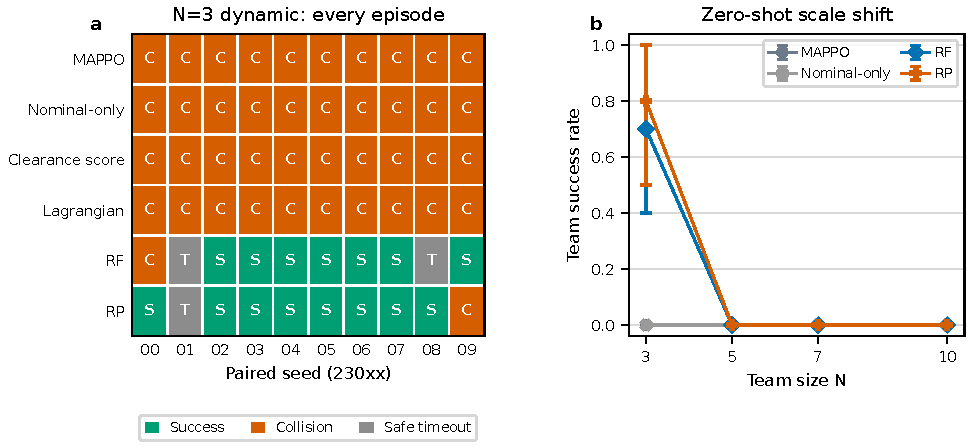
\includegraphics[width=0.985\linewidth]{fig02_mechanism_screening.pdf}
\caption{\textbf{Stage-I mechanism screen.} (a) Terminal outcomes for the ten paired $N=3$ dynamic episodes. S, C, and T denote success, collision, and collision-free timeout. (b) Zero-shot scale shift in the dynamic scenario. Error bars are episode-level bootstrap 95\% intervals.}
\label{fig:screening}
\end{figure}

The independent safety-budget sweep distinguishes hard rejection from soft penalization. As $d_s$ increases from 0.8 to 1.6~m, RF success rises from $6/10$ to $8/10$ and $9/10$, while collision falls from $3/10$ to $1/10$. RP instead records $6/10$, $5/10$ and $7/10$ successes and $4/10$, $3/10$ and $3/10$ collisions. This difference is consistent with the intervention definitions: increasing $d_s$ directly tightens the RF admissible set but changes only one term in RP's competing score. It does not prove that the two variants are statistically ordered.

All ten one-at-a-time RP coefficient perturbations retain $8/10$ success; eight retain $1/10$ collision, whereas weaker residual penalty or stronger goal progress yields $2/10$ collisions. These observations support the direction of the residual account but cannot establish coefficient invariance from ten seeds. The discrete effect vanishes in dense $N=3$ and dynamic $N\geq5$ cells, where every arm collides in every episode. This negative result motivates the continuous transfer test and prevents the discrete screen from being read as evidence of scale.

\subsection{Continuous graph-CBF improves the paired dynamic cells}
The mechanism transfers to continuous control in the two prespecified dynamic cells. Local graph-CBF reduces collision from $100\%$ under the compute-matched MAPPO adaptation to $12.6\%$ at $N=3$ and $31.0\%$ at $N=5$ (Table~\ref{tab:dynamic}); team success rises from $0\%$ to $29.8\%$ and $15.6\%$. Graph-CBF is safe while MAPPO collides in 437 of 500 paired $N=3$ episodes and 345 of 500 paired $N=5$ episodes, with no reverse discordance. Holm-adjusted exact $p$ values are $1.13\times10^{-131}$ and $2.79\times10^{-104}$. A secondary mixed-effects model assigns the MAPPO indicator a collision log-odds mean of 8.59 (posterior s.d. 0.81), consistent with the paired analysis without broadening its estimand.

\begin{table*}[t]
\caption{Dynamic-scenario outcomes. Values are percentages with hierarchical-bootstrap 95\% intervals. Learned policies use $n=500$ episodes per cell. Distributed CBF uses $n=100$.}
\label{tab:dynamic}
\centering
\small
\begin{tabular}{lcccc}
\toprule
& \multicolumn{2}{c}{$N=3$} & \multicolumn{2}{c}{$N=5$} \\
Controller & Success & Collision & Success & Collision \\
\midrule
Graph-CBF (local) & 29.8 [11.2,53.0] & 12.6 [6.6,18.8] & 15.6 [3.6,33.4] & 31.0 [24.2,39.2] \\
Distributed CBF & 10.0 [5.0,16.0] & 14.0 [8.0,21.0] & 1.0 [0.0,3.0] & 38.0 [29.0,47.0] \\
MAPPO adaptation & 0.0 [0.0,0.0] & 100 [100,100] & 0.0 [0.0,0.0] & 100 [100,100] \\
\bottomrule
\end{tabular}
\end{table*}

The distributed-CBF control localizes the source of this gain. In dense $N=3$, graph-CBF achieves $65.6\%$ success and $3.4\%$ collision, compared with $57\%$ and $5\%$ for distributed CBF. In dynamic $N=3$, collision is similar ($12.6\%$ versus $14\%$), but success rises from $10\%$ to $29.8\%$. Thus, projection alone can limit contacts, whereas the learned message-conditioned residual primarily restores progress. This comparison does not imply uniform dominance across cells.

\subsection{Scale shift reveals the mechanism boundary}
Scale exposes the boundary of the transferred mechanism (Fig.~\ref{fig:scale}). In dynamic scenes, local graph-CBF success falls from $29.8\%$ at $N=3$ to $15.6\%$, $9.8\%$ and $2.8\%$ at $N=5,7,10$, while collision rises from $12.6\%$ to $31.0\%$, $37.4\%$ and $55.0\%$. Dense-layout success remains higher at intermediate sizes ($65.6\%$, $41.0\%$ and $36.0\%$ for $N=3,5,7$) but collapses to $3.2\%$ at $N=10$. In the withheld dense $N=12$ layout, all four learned-policy families record $0\%$ success and $100\%$ collision.

\begin{figure*}[t]
\centering
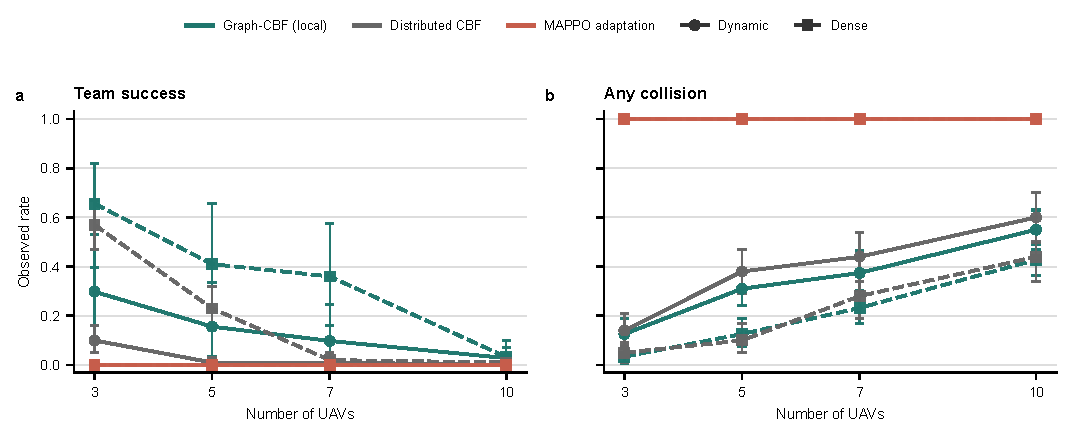
\includegraphics[width=0.985\linewidth]{fig05_continuous_scale.pdf}
\caption{\textbf{Continuous-control scale test.} Team success (a) and any collision (b) for dynamic and dense scenarios. Points are observed rates. Error bars are hierarchical-bootstrap 95\% intervals. Learned-policy cells contain five training seeds and 100 evaluation seeds ($n=500$). Distributed-CBF cells contain 100 evaluation seeds.}
\label{fig:scale}
\end{figure*}

Intervention logs suggest why. Local graph-CBF averages 244 projected commands per $N=3$ episode and 655 per $N=10$ episode; at least one constraint remains unresolved in $95\%$ and $100\%$ of episodes, respectively. The safety layer changes from an occasional correction into a dominant policy action. Hover can remove an instantaneous violation but cannot select a multi-step route through congestion. This diagnostic is consistent with a horizon-limited failure but does not prove that horizon is the sole cause.

\subsection{Privileged observations do not remove scale failure}
More information does not remove this boundary (Fig.~\ref{fig:information}). Averaged over five scenarios, local versus privileged collision rates are $16.1\%$ versus $15.0\%$ at $N=3$, $32.8\%$ versus $34.9\%$ at $N=5$, $42.7\%$ versus $39.0\%$ at $N=7$, and $57.0\%$ versus $48.8\%$ at $N=10$. Mean team-success differences never exceed 1.7 percentage points. Privileged visibility reduces collision at larger $N$ but does not restore completion, and both variants fail at $N=12$. Information scarcity is not the only explanation; the data do not establish equivalence between local and privileged actors.

\begin{figure*}[t]
\centering
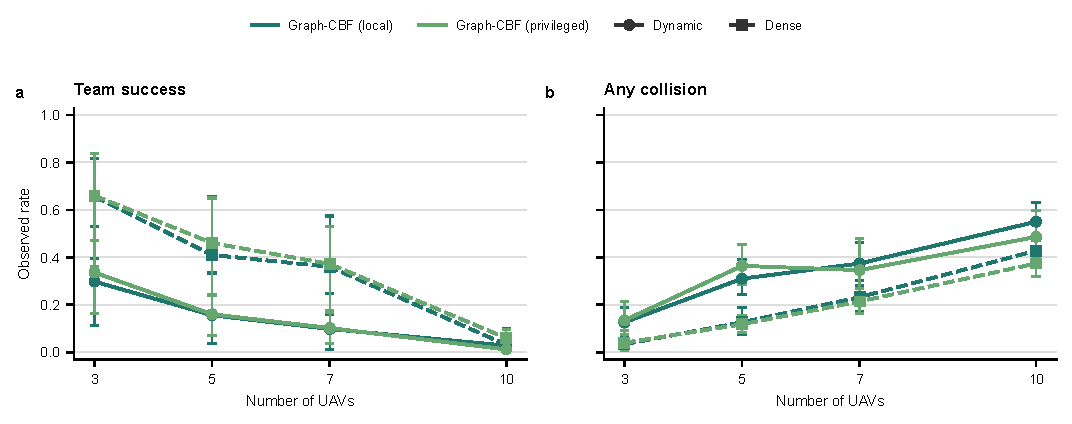
\includegraphics[width=0.985\linewidth]{fig06_information_ablation.pdf}
\caption{\textbf{Information-symmetry ablation.} Local and privileged graph-CBF team success (a) and collision (b) under dynamic and dense conditions. Architectures and training budgets are matched. Only actor visibility changes. Error bars are hierarchical-bootstrap 95\% intervals.}
\label{fig:information}
\end{figure*}

\subsection{PX4 validates the controller interface, not mission safety}
All 400 PX4 SIH runs return telemetry without runtime error or inter-UAV contact during the 3-s Offboard window. Across the four policy--size cells, median maximum velocity-tracking error ranges from 1.65 to 1.75~m/s; median episode-level 95th-percentile send latency ranges from 2.38~ms at $N=3$ to 3.13~ms at $N=5$ (Fig.~\ref{fig:px4}). Both command streams therefore traverse the same 10-Hz multi-instance flight-stack interface. The initial separation is large and the flight dynamics contain no buildings or moving-obstacle contacts, so 100\% interface completion is neither navigation success nor mission-safety evidence.

\begin{figure*}[t]
\centering
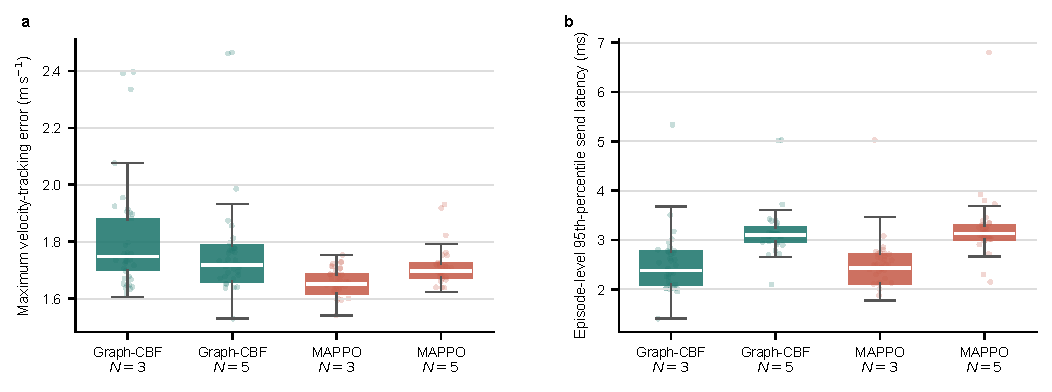
\includegraphics[width=0.985\linewidth]{fig07_px4_interface.pdf}
\caption{\textbf{PX4 SIH interface validation.} Maximum velocity-tracking error (a) and episode-level 95th-percentile command-send latency (b) over 100 runs per policy--size cell. Boxes show the median and interquartile range; whiskers extend to 1.5 times the interquartile range and faint points show a fixed random subset of runs.}
\label{fig:px4}
\end{figure*}

\section{Discussion}

The two stages support one bounded mechanism-level conclusion. Under a shared evaluator, Stage I excludes nominal progress, instantaneous clearance and one Lagrangian cost as sufficient explanations for the observed small-team dynamic gains. Stage II changes the action space, information structure and controller implementation, yet preserves the qualitative effect of rejecting predicted barrier violations. This cross-implementation agreement is more informative than a score increase within either stage because most implementation details change while the proposed invariant is retained.

The same evidence identifies where residual rejection stops being sufficient. Larger teams generate overlapping half-spaces and route conflicts that cannot be resolved one step at a time. As projection frequency rises, the nominal actor ceases to be the primary closed-loop policy; the safety layer repeatedly overrides it and hover converts imminent contact into deadlock or delayed collision. Privileged visibility lowers collision at $N=10$ without recovering completion, showing that additional state alone does not repair the missing planning horizon. A natural next test is to couple graph certificates to multi-step or optimization-based planning, rather than further tuning a one-step score.

The universal collision rate of the MAPPO adaptation must be interpreted against its deliberately short, compute-matched budget. It identifies a weak baseline in this implementation, not a general failure of MAPPO in multi-UAV navigation. The defensible contrast is narrower: with seeds, transitions and evaluator fixed, the combined addition of graph aggregation, barrier supervision and command projection changes terminal safety. Because these three components are not separately ablated, the continuous experiment transfers the mechanism hypothesis but does not isolate the contribution of each component.

Auditability depends on responsibility allocation as much as on stored files. The automated loop implemented candidates, executed common tests, orchestrated experiments, aggregated records, generated figures and produced an initial draft. Human researchers fixed terminal labels, primary contrasts, evidence boundaries, citations and final interpretation. Preventing the candidate generator from redefining success after observing outcomes is a scientific control condition, not merely a disclosure convention.

\section{Limitations}

The stages share a barrier-rejection principle but are not algorithmically equivalent. Stage I uses full simulator geometry and discrete one-step prediction; Stage II uses analytic local pairwise half-space projection around a learned graph actor. Neither is an implementation-equivalent reproduction of GCBF$+$ or DGPPO, and neither establishes forward invariance under model mismatch.

Only five independent training seeds and 9,216 transitions per run were available. Hierarchical intervals and paired tests represent training- and evaluation-seed variation within this design, but cannot substitute for longer training, broader layouts or independently implemented baselines. The distance-based target, myopic projection and hover fallback also confound graph aggregation, barrier supervision and projection. Structural ablations are required before attributing the continuous gain to any one of them.

The simulator uses simplified dynamics and fixed urban geometry. PX4 SIH establishes command-path execution, timing, telemetry capture and multi-instance operation over three seconds, but does not instantiate obstacle contacts, long-horizon completion, sensor noise or hardware aerodynamics. Hardware-in-the-loop and outdoor tests under partial observation remain outside the evidence boundary.

\section{Conclusion}

An evidence contract converted generated controller candidates into an independently recomputable mechanism test. Discrete screening and continuous transfer jointly support barrier-residual rejection in small-team dynamic avoidance. Scale failure, privileged-observation ablation and the limited PX4 interface test show that this mechanism is insufficient for scalable or deployment-level safety. The central result is the traceable path from hypothesis to evidence, attempted falsification and explicit boundary, rather than an unconditional safety claim.

\bibliography{uav_ai_discovery}
\bibliographystyle{icais_conference}

\clearpage
\appendix
\raggedbottom
\section{Artifact availability}

Code, environment records, trained checkpoints, the 44,000 simulation episode records, PX4 episode summaries and telemetry, figures, logs and verification hashes are publicly available at \url{https://github.com/Jackson27249/ai-assist-multi-UAV-control} (release v1.0.0). These records permit independent recomputation of the reported aggregates. Low-level PX4 ULog binaries, duplicated sharded copies and per-episode renderings are excluded from the Git repository because they are not inputs to the reported aggregate calculations; the public manifest records the released snapshot.

\section{Responsibility Allocation}

\begin{table}[H]
\caption{Responsibility allocation under the evidence contract.}
\label{tab:responsibility}
\centering
\small
\begin{tabular}{L{0.25\linewidth}L{0.65\linewidth}}
\toprule
Role & Responsibility \\
\midrule
Human researchers & Research question and evidence boundary. Simulator and compute. Terminal labels. Review of mechanism mapping, statistics, citations, and final conclusions. \\
Automated loop & Repository inspection. Candidate implementation. Common-evaluator testing. Experiment orchestration. Aggregation. Visualization. Initial manuscript drafting. \\
\bottomrule
\end{tabular}
\end{table}

\section{Prompt Audit Record}

The following normalized prompt specifications record the operational constraints supplied to the automated loop. They are protocol-level inputs rather than a claim that the loop independently chose the research question, terminal labels, or final interpretation. Each prompt was constrained to retain rejected variants and source records. No prompt specified a target success rate, collision rate, or preferred conclusion.

\begin{enumerate}
\item \textbf{Evidence contract.} ``Lock the controller definitions, seed lists, terminal-label evaluator, aggregation rule, and source-artifact paths before analysis. Treat collision, collision-free timeout, and team success as distinct outcomes. Retain every evaluated candidate and report any claim only when its episode-level evidence can be recomputed.''

\item \textbf{Mechanism screen.} ``Use the observed inter-UAV failure labels to construct safety variants around one unchanged goal-progress controller. Include MAPPO, nominal-only, clearance, Lagrangian, hard residual filtering, and soft residual penalization. Pair all variants on the same initial-state, wind, obstacle-motion, and dropout realizations. Do not replace terminal labels with a proxy-cost improvement.''

\item \textbf{Falsification and inference.} ``Evaluate the prespecified size--scenario matrix, an independent safety-budget sweep, and one-at-a-time RP coefficient perturbations. Export episode records before aggregation. Estimate binary-rate intervals by bootstrap and use exact paired tests for the prespecified dynamic contrast. State when intervals or paired tests do not rank alternatives.''

\item \textbf{Continuous transfer.} ``Translate the residual-rejection hypothesis to simultaneous continuous control using local graph observations and barrier projection. Match training budget, critic access, disturbance cells, and evaluation seeds across local graph-CBF and MAPPO adaptations. Add a privileged-observation ablation, but keep simulator geometry out of local actors and distinguish an interface test from urban obstacle-safety evidence.''

\item \textbf{Claim audit.} ``Recompute tables and figures from retained records, inspect discrepancies against the locked terminal labels, and write a bounded conclusion. Separate supported mechanism evidence, negative scale results, and untested deployment claims. Attribute research-question selection, evidence boundaries, and final interpretation to human researchers.''
\end{enumerate}

\section{Mechanism-Screening Algorithm}

\begin{algorithm}[H]
\caption{Mechanism screening under the evidence contract}
\label{alg:loop}
\begin{algorithmic}[1]
\Require fixed baseline $\pi_0$, simulator $\mathcal E$, candidate set $\mathcal M$, paired seeds $\mathcal S$
\State attribute baseline terminal failures by collision type
\For{each $m\in\mathcal M$ that passes the common evaluator}
  \State instantiate controller $\pi_m$ and lock its configuration
  \For{each experimental cell and $s\in\mathcal S$}
    \State evaluate $\pi_m$ and store terminal labels and diagnostics
  \EndFor
  \State recompute aggregates and retain failed as well as favorable variants
\EndFor
\State admit only claims supported by locked configurations and recomputable records
\end{algorithmic}
\end{algorithm}

\section{RP coefficient specification}
\label{app:rp}
For Eq.~\ref{eq:rp_score}, the prespecified values were $\beta_g=8$, $\beta_\rho=12$, $\epsilon=0.01$, $\beta_n=0.03$, $\beta_c=0.12$, and $d_{\max}=3$. These are dimensionless weights applied after normalization of progress, residual and clearance. They were selected as a transparent starting scale, not tuned against held-out outcomes; each coefficient was perturbed by $\pm50\%$ one at a time in the sensitivity experiment.

\section{Stage-I Falsification Detail}

\begin{figure}[H]
\centering
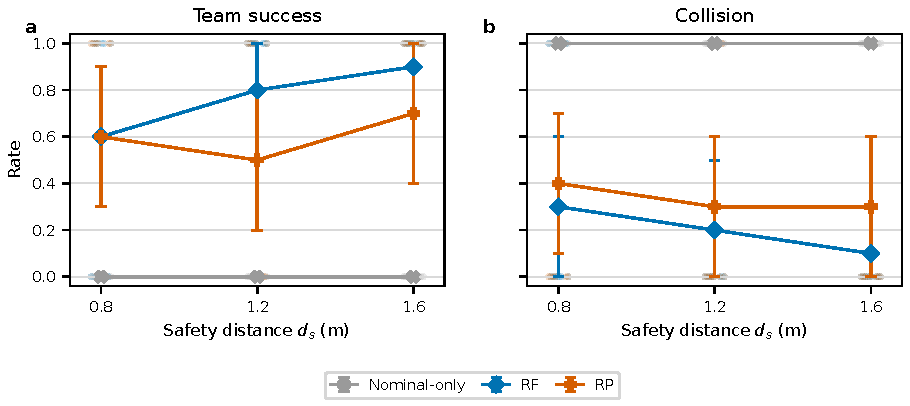
\includegraphics[width=0.985\linewidth]{fig03_independent_budget_sweep.pdf}
\caption{Independent $N=3$ dynamic safety-budget sweep. Faint points are binary episode outcomes; estimates and error bars are observed rates and bootstrap 95\% intervals ($n=10$ per controller--budget cell).}
\label{fig:budget}
\end{figure}

\begin{figure}[H]
\centering
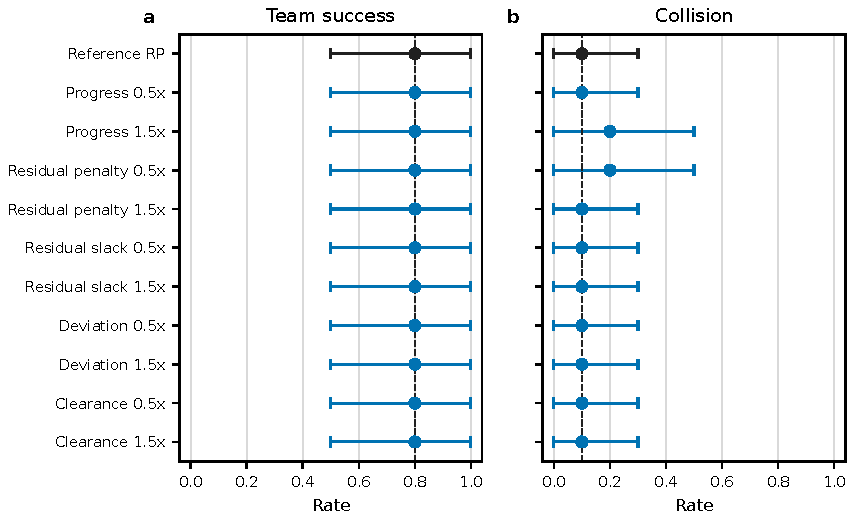
\includegraphics[width=0.88\linewidth]{figS1_rp_weight_sensitivity.pdf}
\caption{RP one-at-a-time coefficient sensitivity in the dynamic $N=3$ cell. Each perturbation uses the same ten paired seeds; points and bars are observed rates and bootstrap 95\% intervals.}
\label{fig:sensitivity}
\end{figure}

\section{Complete Continuous-Policy Summary}

\begin{table}[H]
\caption{Outcomes averaged equally over the five in-distribution scenarios. Each learned entry contains 2,500 episodes (five training seeds, 100 evaluation seeds, five scenarios); distributed CBF contains 500 episodes. Values are team success/collision percentages.}
\label{tab:allpolicies}
\centering
\small
\begin{tabular}{lcccc}
\toprule
Controller & $N=3$ & $N=5$ & $N=7$ & $N=10$ \\
\midrule
Distributed CBF & 23.2/22.8 & 9.6/38.2 & 2.0/49.2 & 0.6/59.4 \\
Graph-CBF (local) & 37.3/16.1 & 22.0/32.8 & 13.8/42.7 & 1.7/57.0 \\
Graph-CBF (privileged) & 37.4/15.0 & 21.2/34.9 & 15.5/39.0 & 2.0/48.8 \\
MAPPO adaptation (local) & 0.0/100 & 0.0/100 & 0.0/100 & 0.0/100 \\
MAPPO adaptation (privileged) & 0.0/100 & 0.0/100 & 0.0/100 & 0.0/100 \\
\bottomrule
\end{tabular}
\end{table}

\section{Statistical Details}

The primary exact McNemar comparisons use collision labels from matched training and evaluation seeds in the dynamic cells. For $N=3$, the discordant counts are 0 graph-CBF-collision/MAPPO-safe pairs and 437 graph-CBF-safe/MAPPO-collision pairs; the raw and Holm-adjusted $p$ values are $5.64\times10^{-132}$ and $1.13\times10^{-131}$. For $N=5$, the corresponding counts are 0 and 345, with raw and adjusted $p=2.79\times10^{-104}$. No learned-policy comparison is presented as an algorithm-level benchmark beyond the fixed training budget.

\section{Complete Successful Urban-Task Trajectories}

Figures~\ref{fig:urbancase3} and~\ref{fig:urbancase5} show complete local graph-CBF trajectories from initialization to terminal task success in the dense urban layout. Both use training seed 1104 and evaluation seed 31002 so that team size is the only changed index. The displayed episodes include all seven buildings and both moving obstacles; every UAV terminates within the 0.65-m goal radius without collision. These simulation cases provide the complete mission-path evidence, whereas the PX4 experiment in the main text remains an interface-only validation.

\begin{figure}[H]
\centering
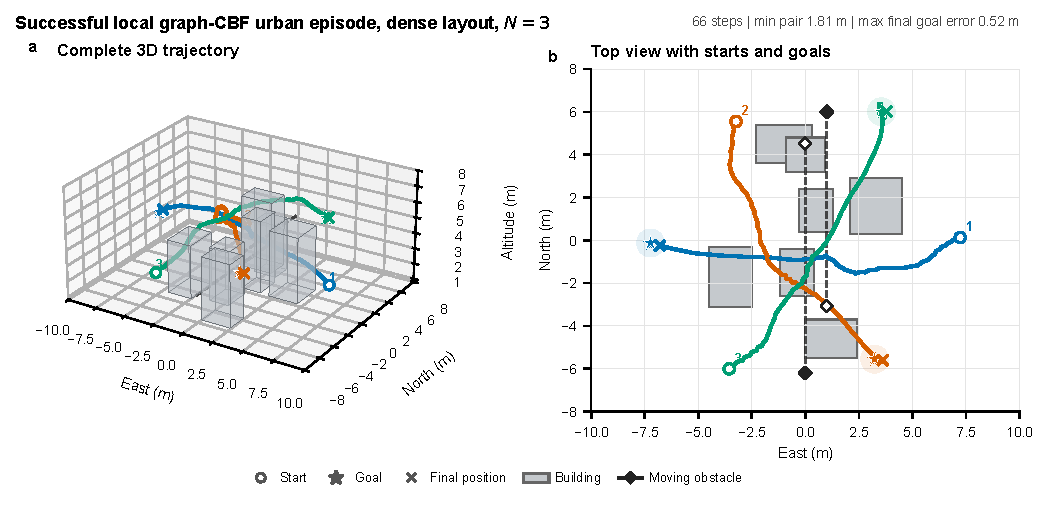
\includegraphics[width=0.985\linewidth]{figS4_gcbf_n3_dense_success.pdf}
\caption{Complete successful dense-layout episode at $N=3$. All trajectories are shown over 66 control steps (16.5~s). Open circles mark starts, stars mark goals, crosses mark terminal positions, and shaded goal disks show the 0.65-m success radius in top view. The minimum inter-UAV distance is 1.81~m and the maximum terminal goal error is 0.52~m.}
\label{fig:urbancase3}
\end{figure}

\begin{figure}[H]
\centering
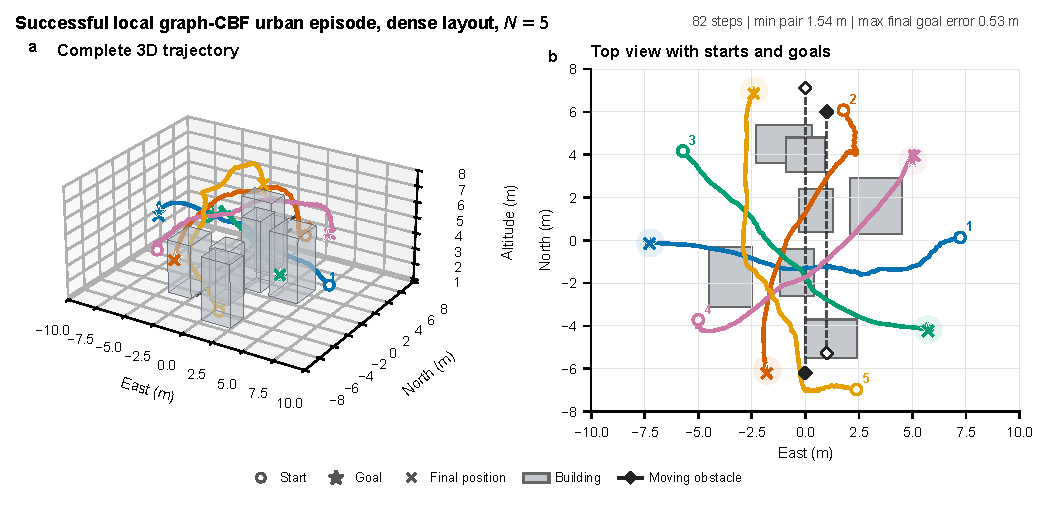
\includegraphics[width=0.985\linewidth]{figS5_gcbf_n5_dense_success.pdf}
\caption{Complete successful dense-layout episode at $N=5$. All trajectories are shown over 82 control steps (20.5~s), with the same start, goal, terminal-position, building, and moving-obstacle encodings as Fig.~\ref{fig:urbancase3}. The minimum inter-UAV distance is 1.54~m and the maximum terminal goal error is 0.53~m.}
\label{fig:urbancase5}
\end{figure}

\section{Additional Environment Detail}

The workspace is $[-10,10]\times[-8,8]\times[0.8,8.0]$~m. The standard layout contains four axis-aligned buildings and the dense layout adds three central-route buildings; the withheld dense layout adds an eighth structure. Dynamic scenarios contain two obstacles initialized near $(0,-6.2,2.6)$ and $(1,6,4)$~m and moving at 0.65 and $-0.55$~m/s along $y$. Wind-scale and communication-dropout pairs for static, dynamic, dense, wind, dropout, and out-of-distribution dense scenarios are $(0.10,0.05)$, $(0.25,0.08)$, $(0.30,0.10)$, $(0.65,0.15)$, $(0.40,0.45)$, and $(0.45,0.25)$.

\end{document}
